\chapter{Concept and Design}
\label{cha:conceptanddesign}

DC3 dashboard has 3 different types of personas - Company, Customer and Postman. Hence we had to design the system differently for each user persona. Our front end application is a Single Page Application (SPA) using react JS. Our back-end is developed by using Node JS leveraging Express framework. 

\section{Architecture}
DC3 follows a modular approach for the whole system. As shown in the bigger picture, entry point for the system is social login, Google in this case. we are using passportJS which can be used to integrate other social strategies e.g. GitHub, Facebook as well. Furthermore, passport does provide local strategy as well where we can configure local database as well for authentication and authorization. This feature would be useful when we different vendors does deploy their own instances of the diLLas service and want to authorize the existing customer base from their own system. we have detailed overview for google authorization explained later as well 

\begin{figure}[!ht]
	\centering
	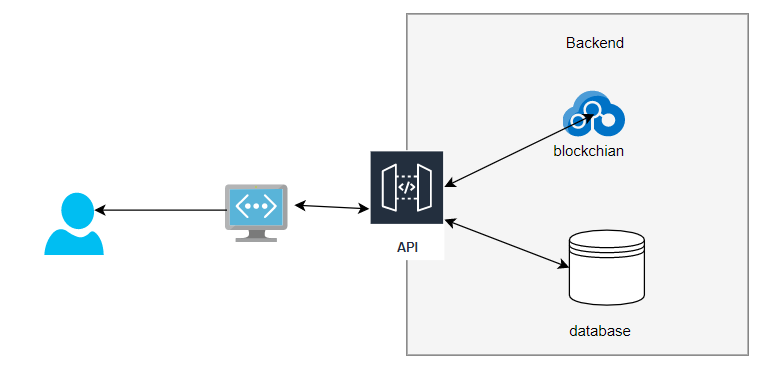
\includegraphics[width=1 \textwidth]{images/bigger_picture.png}\\
	\caption{System Architecture(abstract view)}
	\label{fig:System Architecture(abstract view)}
\end{figure}

Once user is logged-in, for example from browser, an access-token is stored into the local session storage for being used on the front end SPA (Single Page Application) react app.  This token is used for further communication between front-end and back-end. It contains user profile and authorization info. This info is leveraged to protect the different endpoints on the server side and provide related data based on the user type. For example, when a customer hits the /packages endpoint he will be able to see his own packages only but when a company user hits the same endpoint, he will get all the company level packages in the response.

\section{Authentication and Authorization with Google}
Authentication is a vital part of the project and most real world applications need authentication and authorization. While authentication identifies some entity as a valid user, authorization defines the actions that the user is allowed to perform, based on his/her roles and rights. There are many solutions to provide for authentication or authorization in an application and we had two major choices,

\begin{itemize}
\item First one was to keep user state management on Redux.
\item Second was to use a Facebook or a Google Authentication integration with our application.
\end{itemize}

We chose to go with the second choice as it was a new learning for the team to integrate it with our application, reduces the burden for the users to register themselves rather directly sign in with their Google accounts and more importantly because it provides back-end services to securely authenticate users, paired with easy-to-use client SDKs. It can authenticate users using passwords and federated identity provider credentials. 

In our application, once the user clicks on the Google authenticate button,it directs the user to Google's OAuth 2.0 server, which requests access to the user's meta data from the Google drive with a read only scope. Further after granting or denying the access to the user, is then redirected to the original page, which pareses the access token from the string. The page then uses this access token to make  a simple API request which calls the Drive API's to retrieve the information about the authorized user's Google account. If this request is successful then the API response is logged in the browser.
For the first time user's we check our local database to determine the existence and add the user to our database if the user name does not exist and fill in the vital information using the above fetched information from the authorized user's Google account. If the user name exists before hand, we validate the token from the server side with the OAuth2.0 provider and once validated, a JSON Web Token (JWT)  is produced to securely provide authorization to the front end.
We use a main component in our database table "Persons" that is "PersonType" component which determines the role given to a user.Based on this value we determine if the user is either a customer,postman or a company representative. The role with the lowest features is the role of a user, which is the value provided by default to the user on first time log in and henceforth the company role has  authorization to upgrade the user to a postman or a company representative. Initial company role setup is done by the admin. The below figure provides a overview of the functioning of the Google authentication and Authorization based on role integrated to our DC3 application.

\begin{figure}[!ht]
	\centering
	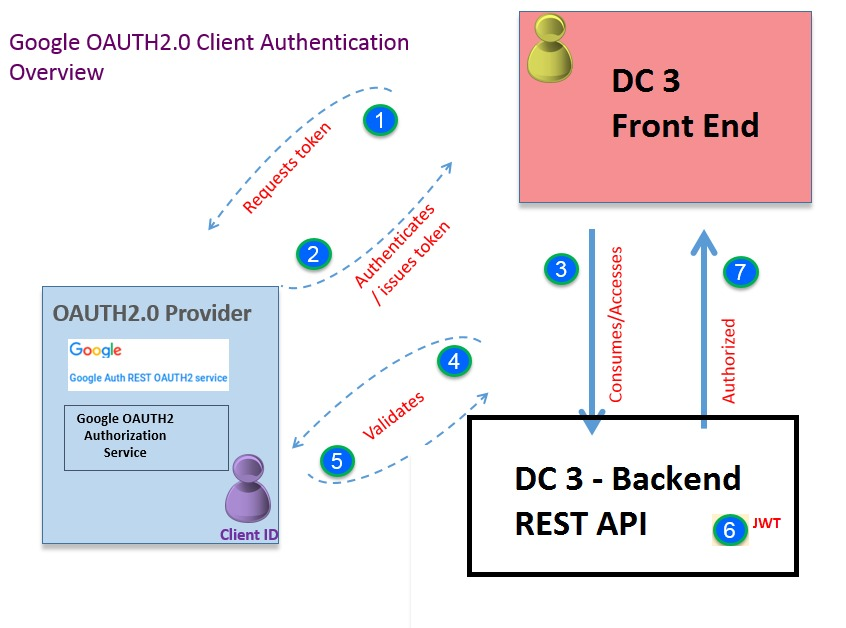
\includegraphics[width=0.5\textwidth]{images/GoogleAuth.jpeg}\\
	\caption{Authentication \& Authorization}
	\label{fig:Authentication and Authorization}
\end{figure}

%pk%


\section{Database Design}
DC3 database has 8 tables. Order, Person, Order History and Order sensors are the major tables while others play an important role as well.  Designs majorly circulate around Orders table. We have normalized the database to avoid storing redundant data e.g. Order and Sensors had many to many relationship so we divided it and created another table, OrderSensors. Let’s understand the philosophy behind each table


\subsection{Company}
The company table is persisting the information about all the companies. It stores the company name and a brief description of the company. 

\begin{table}[!ht]
	%\small
	\centering
	\begin{tabular}{ |l|l|l| }
		\hline
		Id & Int - auto increment & Unique company ID \\
		\hline
		Name & varchar & Company Name \\
		\hline
		Description & varchar & Brief company description \\
		\hline
	\end{tabular}
	\caption{Company table}
\end{table}



\subsection{Address}
Address table is maintaining all kind of address across the whole system, be it order adree or customer home address. Hence it has relationship with Order and Person. Order table has two address Ids, each for pick and delivery address of the order



\begin{table}[!ht]
	%\small
	\centering
	\begin{tabular}{ |l|l|l| }
		\hline
		AddressId  & Int - Autoincrement & \\
		\hline
		StreetAddress  & varchar & \\
		\hline
		City  & varchar &\\
		\hline
		Country  & varchar &\\
		\hline
		PostCode  & int &\\
		\hline
	\end{tabular}
	\caption{Address table}
\end{table}



\subsection{Sensor}
The sensor table is a repository of unique sensors we have available in the system. It will store the names, and different possible thresholds a specific sensors has. It was designed in a generic way to store the different sensors in the same table. 




\begin{table}[!ht]
	\small
	\centering
	\begin{tabular}{ |l|l|l| }
		\hline
		Id  & Int - Autoincrement  & \\
		\hline
		Name  & varchar & \\
		\hline
		MinValue & varchar & Minimum possible reading for the sensor  \\
		\hline
		MaxValue & varchar & Maximum possible reading for the sensor\\
		\hline
		DisplayUnit  & varchar & \\
		\hline
	\end{tabular}
	\caption{Sensor table}
\end{table}


\subsection{Person}
The Person table is storing various kinds of user information. It stores personal information for the company, customer and postman. Additionally, it maintains the social login values for the user. Once a user signs up, it defaults to a customer but admin or company user can change his role to postman or admin (company) user. 

\begin{table}[!ht]
    \begin{center}
    \begin{tabular}{ |l|l|l| } 
    \hline
    Id & Int - auto increment & Unique company ID \\
    \hline
    FullName & varchar & \\
    \hline
    Email  & varchar & \\
     \hline
    Password & varchar & Minimum possible reading for the sensor \\
     \hline
    DateOfBirth & varchar & Maximum possible reading for the sensor \\
     \hline
    PersonType & varchar & Person type e.g. customer, postman or company \\
    \hline
    PersonRole & int & Stores person role or associated company id \\
    \hline
    GoogleProviderId & varchar & Google user-id \\
    \hline
    GoogleAccessToken & varchar & Logged-in user access token\\
    \hline
    \end{tabular}
    \end{center}
    \caption{Person table}
\end{table}



\subsection{Orders}
Orders table is keeping most of the data in the database and it will have a higher churn rate than any other table in the whole system. It stores a lot of referential ids from other tables than actual data e.g. pick \& drop address, person, company. 

\begin{table}[!ht]
\begin{center}
\begin{tabular}{ |l|l|l| } 
 \hline
Id & Int - auto increment & Unique Order ID \\
 \hline

OrderID & Int - AutoIncrement  & \\
\hline
PickAddressID & Int & Pick up address id\\
\hline
DropAddresID  & Int  & Drop address Id\\
\hline
PickDate  & date & Registration or pick up date\\
\hline
ArrivalDate & date & Delivery date\\
\hline
PersonID & int & Package Sender id\\
\hline
ReceiverPersonID & int & Package Receiver id\\
\hline
Status & varchar & E.g. Registered, In-Transit or Delivered\\
\hline
CompanyId & int & Reference for associated company\\

 \hline
\end{tabular}
\end{center}
    \caption{Orders table}
\end{table}

\subsection{OrderSensors}
\begin{table}[!ht]
\begin{center}
\begin{tabular}{ |l|l|l| } 
 \hline
Id & Int - auto increment & Unique company ID \\
 \hline
Name & varchar & Company Name \\
 \hline
Description & varchar & Brief company description \\
 \hline
\end{tabular}
\end{center}
    \caption{OrderSensors table}
\end{table}

\subsection{Incident}
\begin{table}[!ht]
\begin{center}
\begin{tabular}{ |l|l|l| } 
 \hline
Id & Int - auto increment & Unique company ID \\
 \hline
Name & varchar & Company Name \\
 \hline
Description & varchar & Brief company description \\
 \hline
\end{tabular}
\end{center}
    \caption{Incident table}
\end{table}

\subsection{Database Diagram}
\begin{figure}[!ht]
	\centering
	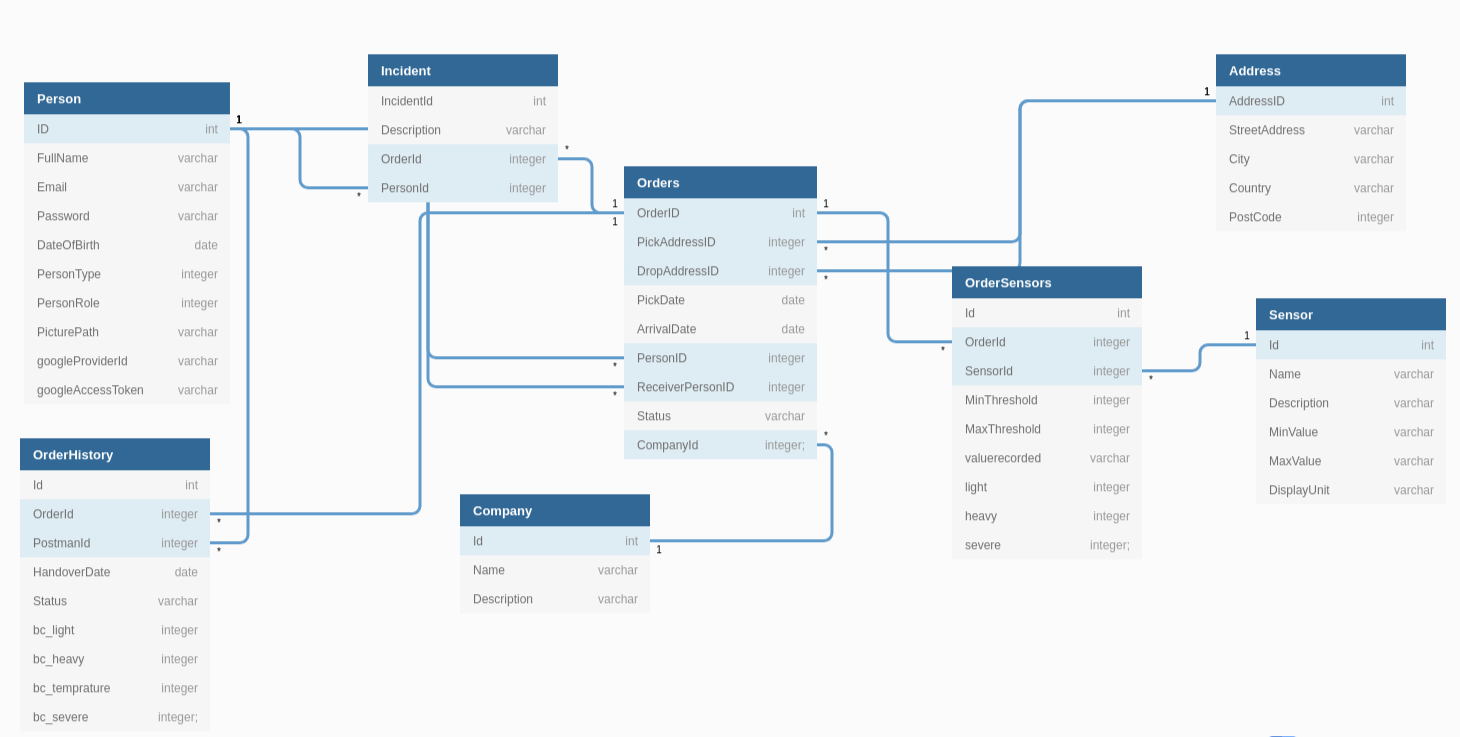
\includegraphics[width=1\textwidth]{images/IOSLDBDiagramlatex.png}\\
	\caption{Database Diagram}
	\label{fig:Database Diagram}
\end{figure}
